\documentclass[a4paper, 12pt]{article}
\usepackage[utf8]{inputenc}
\usepackage[T1]{fontenc}
\usepackage[ngerman]{babel}
\usepackage{geometry}
\usepackage{listings}
\usepackage{xcolor}
\usepackage{hyperref}
\usepackage{helvet}
\usepackage{titlesec}
\usepackage{setspace}
\usepackage{graphicx}

\geometry{a4paper, left=1.5cm, right=1.5cm, top=2cm, bottom=2cm}
\graphicspath{ {./images/} }
% Einstellungen für Code-Listings
\lstset{
    basicstyle=\ttfamily,
    breaklines=true,
    numbers=left,
    numberstyle=\tiny,
    frame=single,
    backgroundcolor=\color{lightgray},
    captionpos=b,
    language=Java % Ändere dies entsprechend deiner Programmiersprache
}

\title{
    Projektdokumentation\\
    Hochschule Mainz - Wi Dual - Praxismodul I
}

\author{
    Bindernagel, Lorenz\\
    Schäfer, Robin\\
    Simic, Darko\\
    Struve, Anika
}

\date{
    \today
}



\begin{document}

    \maketitle
    \tableofcontents
    \newpage

    \onehalfspacing

    \section{Projektidee/ -konzeption}
    
    \subsection{Motivation}
    Design Science: Relevance-Cycle
    Die Motivation des Projekt ist es, einen Plattform für Sammler zu schaffen, die in verschiedenen Themenbereichen Sammlungen besitzen.


    \subsection{Marktanalyse / Technologische Grundlagen}
    Zielgruppe, Marktabgrenzung, theoretische Grundlagen, Literaturüberblick\linebreak
    Design Science: Relevance-Cycle

    \newpage

    \section{Projektplanung / Projektmanagement}
    
    \subsection{Zieldefinition}

    % Wir könnten hier sicherlich auch das Wording Meilensteine nutzen, finde ich besser als Teilergebnisse
    \subsection{Teilergebnisse}
    Die Teilergebnisse lassen sich aus dem Konzept in ~\ref{subsec:designphase} herleiten.
    Grundlegende Teilergebnisse sind die Erstellung des Frontends, die Erstellung des Backends und das Aufsetzen einer Datenbank.
    Neben diesen Zielen, die sich aus der genutzten Architektur ergeben, ist ein weiteres Teilergebnis das Hosten der Website und der Datenbank.
    Für jedes Teilergebnis sind Voranalysen nötig, da die Programmierung einer Webanwendung für das gesamte Team neu ist.
    Als Startpunkt für die Analyse diente GitHub Eduction, welches mit dem Kurs Intro to Web Development einige Tools zum Entwickeln von Websites zur verfügung stellt.
    Die Tools, für die sich durch die Analyse entschieden wurde, werden in ~\ref{subsec:tools} aufgeführt.

    Die Teilergebnisse sind eng miteinander verbunden.
    Essentiell sind hierbei das Hosten der Website und der Datenbank.
    Besonders ohne die Datenbank lässt sich das Backend schwierig entwickeln.
    Das Hosten der Website ist wichtig, um eingebaute Funktionen direkt live testen zu können.
    Die Entwicklung des Frontends, des Backends und der Datenbank ist eng miteinander verzahnt.
    Während Frontend und die Datenbank getrennt voneinander eingerichtet werden können, ist zur Kommunikation der beiden Bereiche das Backend essentiell.
    Während die drei Bereiche einzelne Teilergebnisse bilden, findet der Großteil der Programmierung dieser parallel statt.

    Der Umgang des Frontends ist alles, womit der Nutzer am Ende auf der Website interagieren kann.
    Beispiele hierfür sind die Login-Page, die Ansicht der verschiedenen Sammlungen und die Seite zum Erstellen von Vorlagen.
    Im Anhang befinden sich Mockups, die beim initialen Brainstorming der Projektidee entstanden sind.
    Das Backend soll für die Kommunikation zwischen Frontend und Datenbank verantwortlich sein.
    Es soll die Daten aus der Datenbank an die Benutzeroberfläche übermitteln um diese anzuzeigen.
    Darüber hinaus soll es Änderungen an den Daten, die in der Benutzeroberfläche durchgeführt werden, an die Datenbank kommunizieren.
    Hierbei ist wichtig, dass die Funktionen sicher stellen, dass die Datenbank dynamisch basierend auf Nutzereingaben skaliert wird.
    Die Logik der Website soll in diesem Bereich des Programms festgehalten werden.
    Das Datenbanksystem ist der Ort, an dem die Informationen über Nutzer und Sammlungen hinterlegt werden.
    Die Datenbankform der Vorlagen der Sammlungen werden hier gespeichert.
    Sie muss dabei so eingerichtet sein, dass sie dynamisches hinzufügen und löschen ganzer Tabellen erlaubt.
    % Vllt mal ein Mockup für ein Template erstellen

    \subsection{PSP}
    
    \subsection{Organigramm / Team}
    
    \subsection{Ablaufplanung (Gantt / Netzplan)}
    Wird in YouTrack erstellt.
    
    \subsection{Stakeholderanalyse / Risikoanalyse}
    
    \subsection{Kosten- und Aufwandsplanung}

    \subsection{Tools}\label{subsec:tools}

    \newpage
    
    \section{Projektbericht}
    
    \subsection{Allgemeine Methodik / Vorgehen / Literaturüberblick}
    Bspw.: Business Model Canvas / CRSIP-DM-Cycle / Behavior Driven Development / SCRUM)
    Design Science: Rigor-Cycle
    
    \subsection{Designphase}\label{subsec:designphase}
    Datenmodell / Frontend / Backend
    Design Science: Design-Cycle
    
    \subsection{Prototypvorstellung}
    Design Science: Artefakt

    \newpage
    
    \section{Ergebnis und Fazit}
    
    \subsection{Fazit}
    
    \subsection{Lessons learned}
    
    \subsection{Ausblick}

    \newpage

    \appendix

    \section{Anhang}
    
    \subsection{Mockups}

    \begin{figure}[htbp]
        \centering
        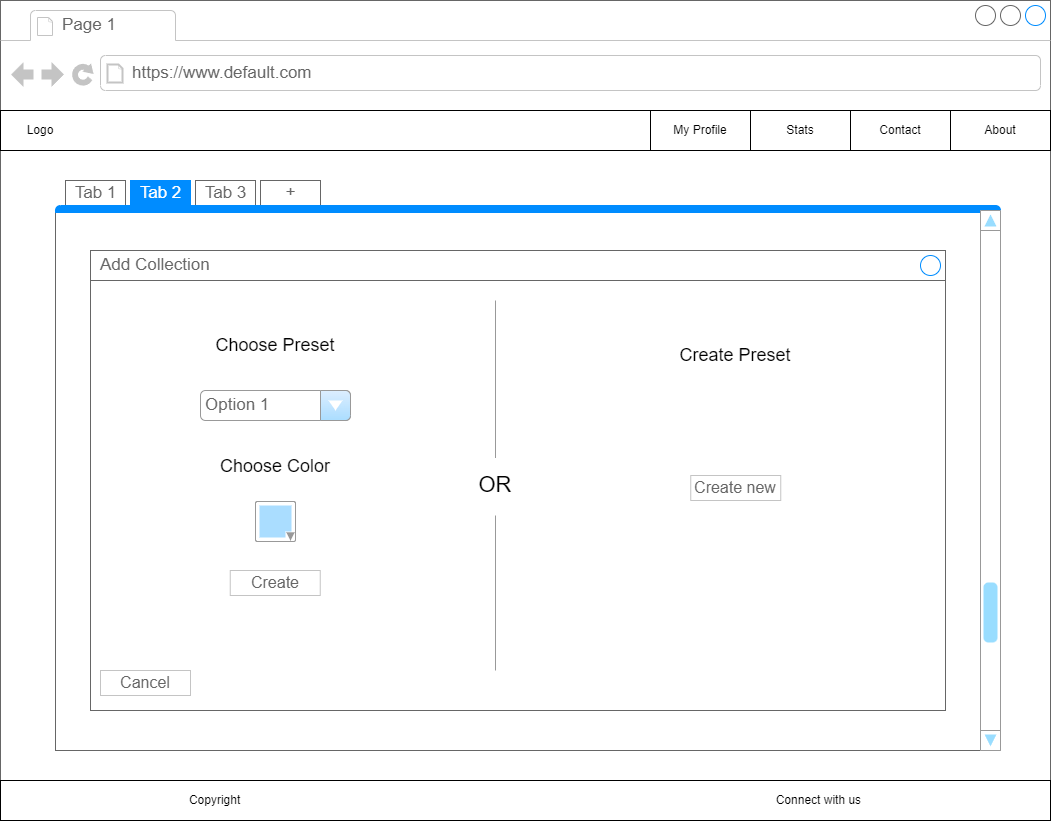
\includegraphics[width=0.6\textwidth]{add_collection_pop_up}
        \caption{'Add Collection' Pop-up}
    \end{figure}    
        
    \begin{figure}[htbp]
        \centering
        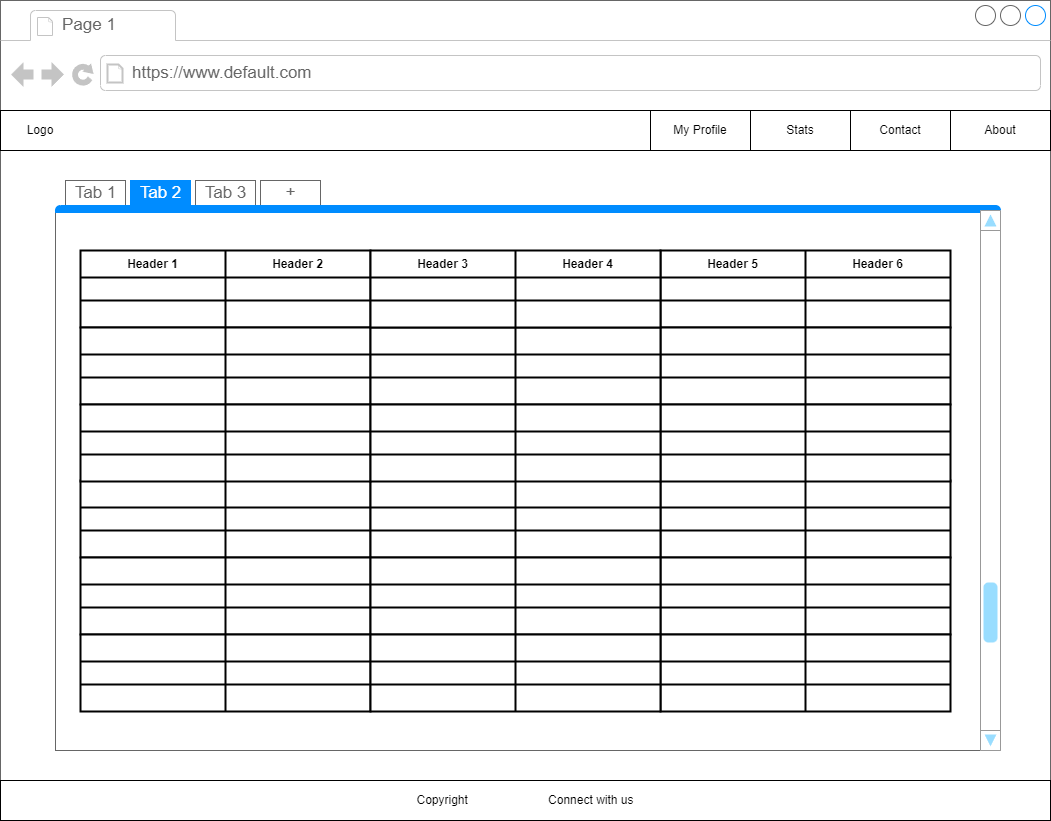
\includegraphics[width=0.6\textwidth]{loggedIn_starting_site}
        \caption{'Logged in' page}
    \end{figure}

    \begin{figure}[htbp]
        \centering
        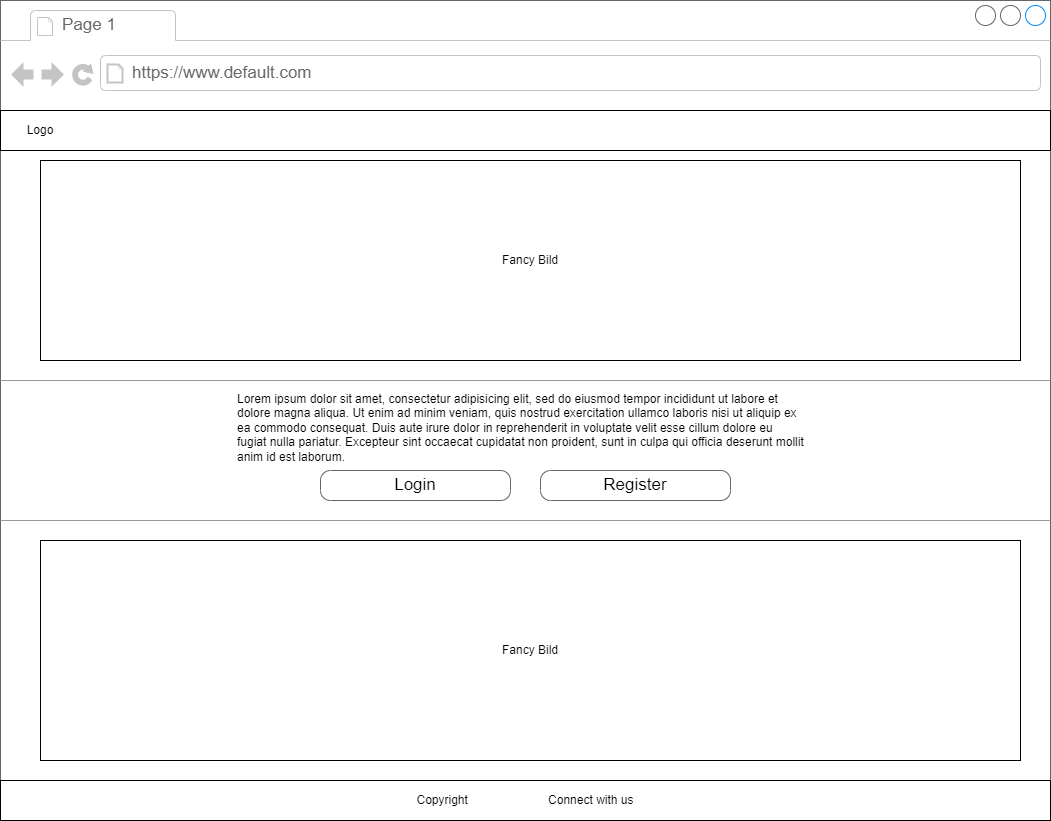
\includegraphics[width=0.6\textwidth]{Starting_site}
        \caption{Starting page}
    \end{figure}

\end{document}
